\documentclass[11pt,a5paper]{memoir}

% usual packages loading:
\usepackage{fontspec}
\setmainfont{Calluna}
\usepackage[autocompile]{gregoriotex} % for gregorio score inclusion
\usepackage{multicol}
\usepackage{graphicx} % support the \includegraphics command and options
\usepackage[pass-fonts=true,program=/usr/bin/lilypond]{lyluatex}
\setlength{\trimtop}{0pt}
\setlength{\trimedge}{0pt}
\settypeblocksize{170mm}{115mm}{*} % Was 101mm in a5
\setulmargins{*}{*}{1.4}
\setlrmargins{*}{*}{1.2}
\setheadfoot{\onelineskip}{2\onelineskip}
\setheaderspaces{*}{.8\onelineskip}{*}
\checkandfixthelayout

\tolerance=1000
\pretolerance=800



\begin{document}

\ 

\vfill

\begin{center}

\textsc{\huge A New Book}

\textsc{\huge of Old Hymns}

\textsc{\large in Latin and English}

chant

polyphony

rounds

a litany

for all the seasons

of the Church's year

\end{center}

\vfill

\eject

\ 

\vfill

First Edition July 2004

Second Edition January 2006

Third Edition October 2007

Compiled by Veronica Brandt http://brandt.id.au.


\eject

\tableofcontents

\newpage

\ 

\vfill

\begin{center}
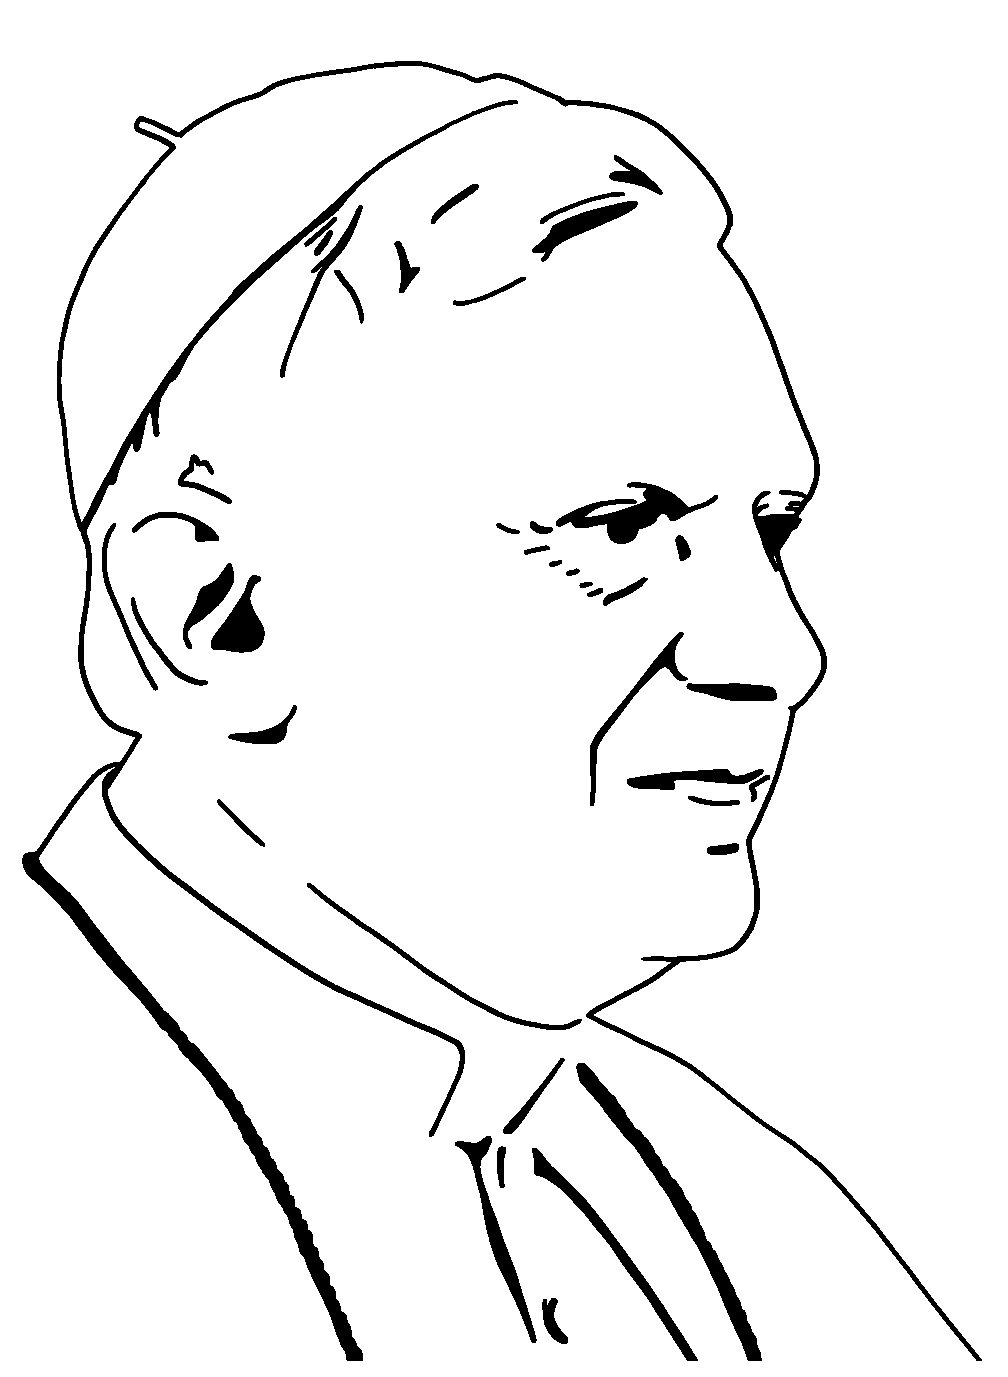
\includegraphics[width=4cm]{images/papab16}
\end{center}

\gregorioscore{gabc/va--oremus_pro_pontifice--solesmes}

\eject

\section{Advent}

\subsection{Conditor Alme Siderum}

\gregorioscore{gabc/hy--conditor_alme_siderum-v1--solesme}

\subsection{Veni O Sapientia}

\input veniosapientia

\subsection{Rorate Caeli}

\gregorioscore{gabc/va--rorate_caeli--solesmes.1}

\gregorioscore{gabc/va--rorate_caeli--solesmes.2}

\gregorioscore{gabc/va--rorate_caeli--solesmes.3}

\gregorioscore{gabc/va--rorate_caeli--solesmes.4}

\gregorioscore{gabc/va--rorate_caeli--solesmes.5}

\section{Christmas}

\subsection{Puer Natus in Bethlehem}

\gregorioscore{gabc/hy--puer_natus_in_bethlehem--solesmes}

\section{Holy Name}

\subsection{Jesu Dulcis Memoria}

\gregorioscore{gabc/hy--jesu_dulcis_memoria--solesmes}


\section{Epiphany}

\section{Candlemas}

\subsection{Lumen ad Revelationem Gentium}

\gregorioscore{gabc/an--lumen_ad_revelationem--solesmes}

\section{Lent}

\subsection{Attende Domine}

\gregorioscore{gabc/va--attende_domine--solesmes}

%\gregorioscore{gabc/va--attende_domine--solesmes.2}

\subsection{Parce Domine}

\gregorioscore{gabc/an--parce_domine--solesmes}

\section{Passiontide}

%Gloria Laus
\subsection{Gloria Laus}

\gregorioscore{gabc/hy--gloria_laus--solesmes.1}


\gregorioscore{gabc/hy--gloria_laus--solesmes.2}


\gregorioscore{gabc/hy--gloria_laus--solesmes.3}


\gregorioscore{gabc/hy--gloria_laus--solesmes.4}


\gregorioscore{gabc/hy--gloria_laus--solesmes.5}


\gregorioscore{gabc/hy--gloria_laus--solesmes.6}


\subsection{Vexilla Regis}

\gregorioscore{gabc/hy--vexilla_regis_prodeunt--solesmes.1verse}


\section{Easter}



\section{Ascension}

\section{Pentecost}

\section{Trinity}

\section{Sacred Heart}

\section{Corpus Christi}

\section{Christ the King}

\section{All Saints}

\section{All Souls}

\section{Marian}

\section{For Peace}

\% The title:
\begin{center}\begin{huge}\textsc{For Peace}\end{huge}\end{center}


\gregorioscore{gabc/an--da_pacem_domine--solesmes}

\bigskip


\section{Thanksgiving}

\section{Kyriale}

\section{Benediction}

\section{Index}

\end{document}
